%! TEX root = /home/simon/Documents/Dagbok_MPPHS_2020-2021/main.tex

\subsection{Måndag 2021-01-18}
Ny LP, nya mögligheter! och en ny uppdaterad kursplan
%! TEX root = /home/simon/Documents/Dagbok_MPPHS_2020-2021/main.tex
\begin{table}[H]
    \centering
    \caption{}
    \label{tab:course_plan_3}
    \begin{tabular}{l|l|l|}
         & Year 1 & Year 2 \\ \hline
        LP1 
        & \begin{tabular}[c]{@{}l@{}}
            \textcolor{compulsory}{Learning from data (C)}\\ \textcolor{compulsory}{Quantum mechanics (B)}\\ \textcolor{compulsory}{Experimental physics (A)}\\ Representation theory
        \end{tabular}
        & \begin{tabular}[c]{@{}l@{}} \textcolor{elective}{Standard model \& beyond (B)}\\ Integration theory\\ Commutative algebra
        \end{tabular} \\ \hline
        LP2
        & \begin{tabular}[c]{@{}l@{}}
            \textcolor{compulsory_elective}{Symmetries (A)}\\ \textcolor{compulsory_elective}{Computational physics (D)}
        \end{tabular}
        & \begin{tabular}[c]{@{}l@{}}
            %\textcolor{elective}{String theory (A)}\\
			\textcolor{elective}{High performance computing}\\
            Algebraic geometry\\
            Foundations of probability theory
        \end{tabular} \\ \hline
        LP3
        & \begin{tabular}[c]{@{}l@{}}
            \textcolor{elective}{Gravitation \& cosmology (A)}\\ Advanced differential calculus
        \end{tabular} &  \\ \hline
        LP4
        & \begin{tabular}[c]{@{}l@{}}
            \textcolor{elective}{Quantum field theory (B)}\\ Vetenskapshistoria (LA)\\ Complex analysis in several variables
        \end{tabular} 
        & \begin{tabular}[c]{@{}l@{}}
           ~
        \end{tabular} \\ \hline
    \end{tabular}
\end{table}


Möte med Thomas idag om masterarbetet, det kommer bli lit! Jag skriver en separat dagbok för masterarbetet.

\bigskip

Kanske high value och se om jag kan sitta med Ludde och dom sen någon dag.

\bigskip

Hade problem med att \verb|:set conceallevel=0| inte fungerade men efter att ha kört\\
\verb|:verbose set conceallevel| upptäckte jag att det var indentLine som satte conceallevel till 2 hela tiden. Så kommenterade ut indentLine.


\subsection{Tisdag 2021-01-19}

Frågor jag har till nästa möte med Thomas:
\begin{itemize}
	\item Arbetet handlar om att göra kvant i GR, det ska ju inte fungera?? what's the deal??
\end{itemize}

\bigskip

Hittade lite najjs info om folds i Vim:
\begin{quote}
The commands zc (close), zo (open), and za (toggle) operate on one level of folding, at the cursor. The commands zC, zO and zA are similar, but operate on all folding levels (for example, the cursor line may be in an open fold, which is inside another open fold; typing zC would close all folds at the cursor).

The command zr reduces folding by opening one more level of folds throughout the whole buffer (the cursor position is not relevant). Use zR to open all folds.
\end{quote}

\bigskip

Jag lade till 
\begin{verbatim}
Plug 'sirver/ultisnips'
Plug 'honza/vim-snippets'
\end{verbatim}
i min \verb|init.vim|. Så nu, om jag skrivir t.ex \enquote{begin} i insert mode, följt av ctrl-j så expanderar Vim det till
\begin{verbatim}
\begin{something}
	
\end{something}
\end{verbatim}
och placerar min cursor på rätt ställe. Detta känns fett användbart men kommer fortfarande skriva många måsvingar, så kommer eventuellt behöva göra ngt åt det. Kombinerat med \verb|dse|/\verb|cse| för delete/change surrounding environment så är jag OP.

Lista på användbara snippets:
\begin{itemize}
	\item \verb|begin| för \verb|\begin{...}...|
	\item \verb|al| för \verb|\begin{align}...|
	\item \verb|item| för \verb|\begin{itemize}...|
	\item \verb|frac| för \verb|\frac{...}{...}|
\end{itemize}
Frågan är om jag kan omdefinera egna snippets? för t.ex \verb|int| blir \verb|\int_{{}}^{{}} {} \: d{} {}|, men jag vill ju ha \verb|\int_{}^{} {} \dd{}{}|.


\subsection{Tisdag 2021-01-19}



\subsection{Tisdag 2021-01-19}

ctrl+r för att byta till night mode i Zathura. Så nu ser mitt workflow riktigt lit ut.
\begin{figure}[H]
	\centering
	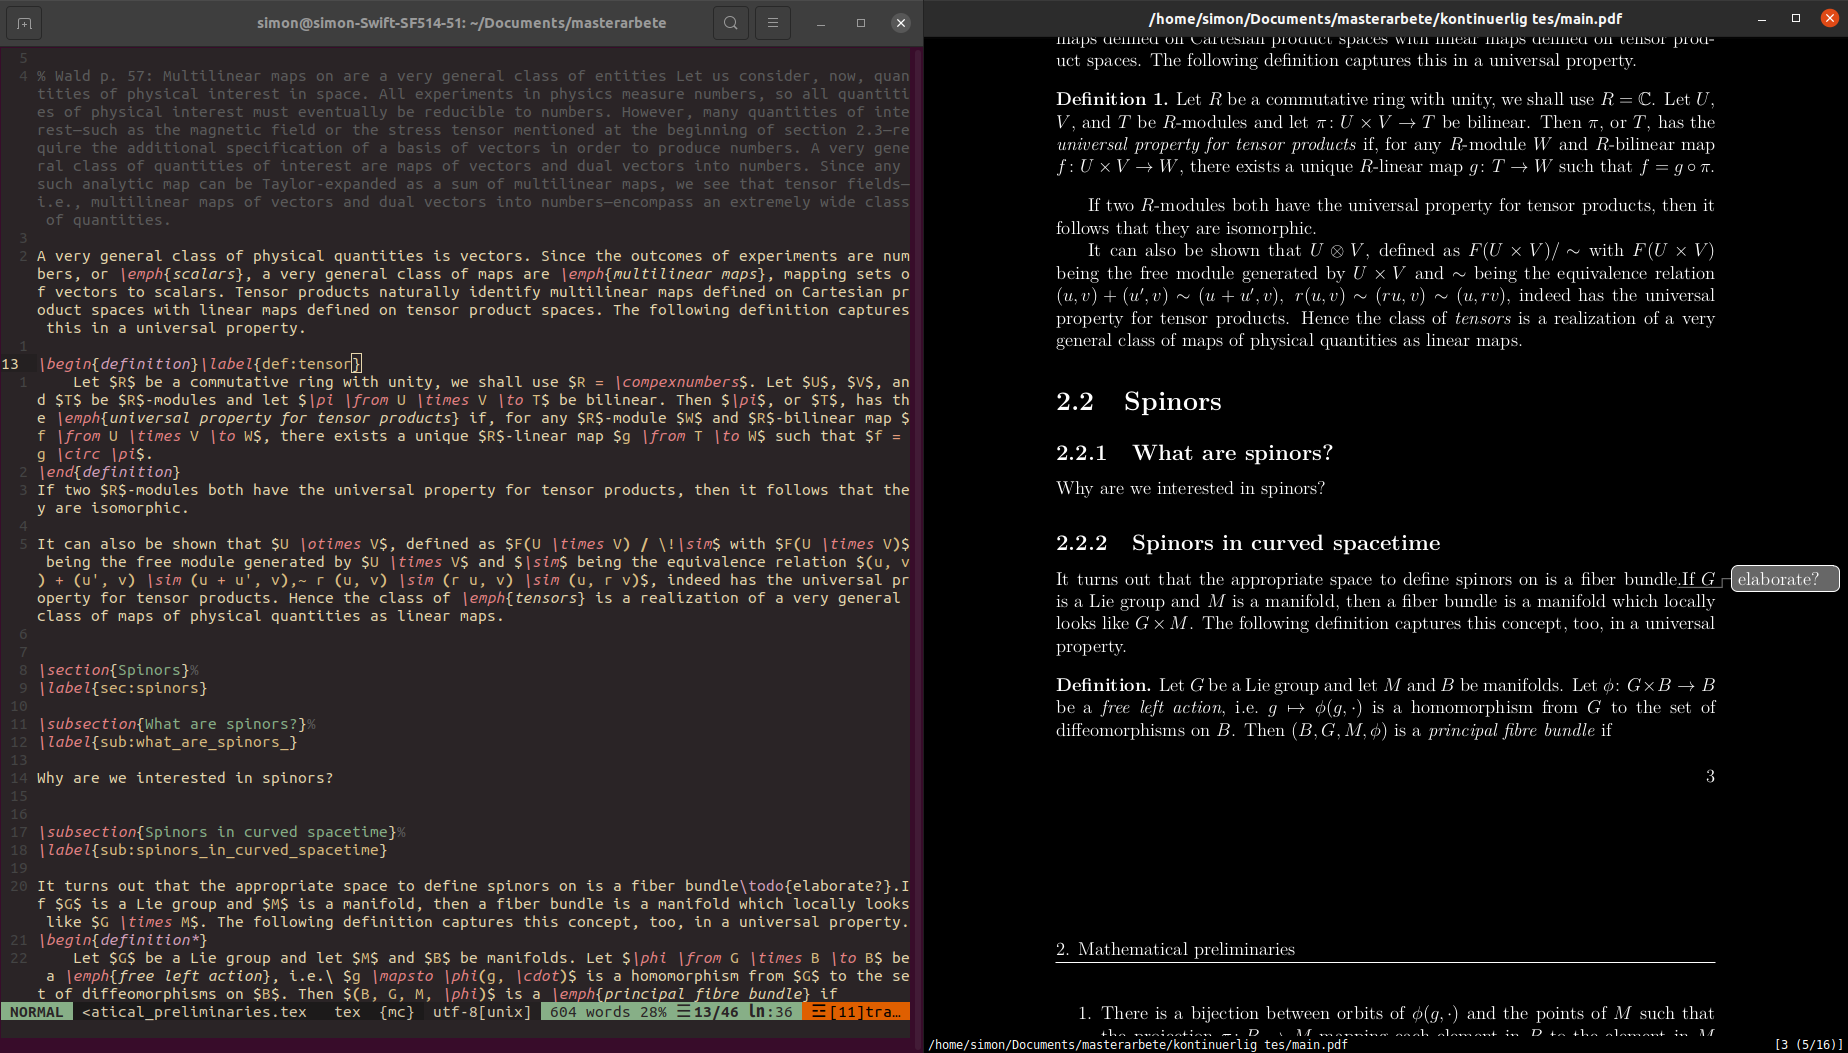
\includegraphics[width=1.0\linewidth]{pics/workflow.png}
	\caption{}%
	\label{fig:workflow}
\end{figure}
Jag gjorde bakgrundsfärgen i night mode lite mildare genom kommandot\\
\verb|:set recolor-lightcolor \#2A2426|
